\documentclass[review]{elsarticle}

\usepackage{lineno}
\usepackage[hidelinks]{hyperref}
\usepackage{mathtools}
\usepackage{adjustbox}

\modulolinenumbers[5]

\graphicspath{ {./figures/} }

\journal{IB200}

%% bibliography styles
%% Harvard
\bibliographystyle{model2-names}\biboptions{authoryear}
%% `Elsevier LaTeX' style
%\bibliographystyle{elsarticle-num}



%%%%%%%%%%%%%%%%%%%%%%%
%% front matter
%%%%%%%%%%%%%%%%%%%%%%%

\begin{document}

\begin{frontmatter}

\title{Fossil-calibrated phylogeny of Onagraceae: patterns of floral and chromosome evolution}

\author[berk]{William A. Freyman\corref{cor1}}
\ead{freyman@berkeley.edu}
\cortext[cor1]{Corresponding author}

\address[berk]{Jepson Herbarium and Department of Integrative Biology, University of California, Berkeley}

\begin{abstract}
blah blah
\end{abstract}

\end{frontmatter}


%%%%%%%%%%%%%%%%%%%%%%%
%% intro
%%%%%%%%%%%%%%%%%%%%%%%

\linenumbers

\section{Introduction}

blah blah

\section{Methods}

\paragraph{Supermatrix assembly} 

I downloaded all available DNA sequences from GenBank release 200 PLN division and
performed an exhaustive all-by-all BLASTn \citep{blast} comparison for sequences in Onagraceae
and Lythraceae.
Using a BLASTn e-value of $1.0e^{-10}$ threshold and a sequence length
percent similarity cutoff of 0.5,
I constructed clusters of putative homologs using a single-linkage hierarchical clustering algorithm.
Subspecies names were removed from all sequences, and all but one sequence of each species was pruned from each cluster.
Clusters that were not phylogenetically informative ($< 4$ taxa) were discarded,
and each cluster was aligned using MUSCLE \citep{edgar2004muscle}. 
The alignments were concatenated by species, and any species that was not present in at least
two clusters was removed from the supermatrix.
Code written to assemble the supermatrix is availabe as the Python module 
Supermatrix Constructor (SUMAC) \citep[\url{https://github.com/wf8/sumac}]{sumac}.



\paragraph{Phylogenetic analyses} 
Maximum likelihood analyses were performed with RAxML-HPC \citep{raxml} on the CIPRES Scientific Gateway \citep{cipres} 
using the rapid bootstrap heuristic and the GTRCAT nucleotide substitution model.
I used the ML tree to select 15 species phylogenetically widely distributed in Lythraceae to act as outgroup; 
all other members of Lythraceae were subsequently removed from the supermatrix before estimating divergence times.
Bayesian estimates of divergence times were inferred using BEAST \citep{beast, beast2} on CIPRES and calibrated with five fossils 
identified with morphological synapomorphies (Table \ref{fossils}).
The \textit{Ludwigia} fossil pollen was dated broadly to the Paleocene \citep{grimsson}, so I set the prior to a normal distribution with a wide 
standard deviation to cover the entire time period.
For all other calibration points I used a lognormal prior distribution with the offset (the minimum age of the node) corresponding to the fossil age.
The BEAST analysis utilized the GTR+$\Gamma$ nucleotide substitution model with a relaxed molecular clock (uncorrelated lognormal model)
and a Yule process tree prior.
The Markov Chain Monte Carlo (MCMC) was run for 100 million generations, sampling every 10 thousand generations.
Tracer v1.6 \citep{tracer} was used to assess the MCMC output for parameter convergence and ensure that the effective sample size for all parameters was above 200.
The first 1000 trees were discarded as burn-in, and the remaining 9000 trees were summarized as a maximum clade credibility tree with mean divergence times. 

\begin{table*}
   \begin{adjustbox}{max width=\textwidth}
      \begin{tabular}{lllllll}
         \hline
         Group & Age (Mya) & Prior Distribution & Mean & SD & Offset & Reference \\ \hline
         \textit{Circaea} (Onagraceae) & 12 & lognormal & 0.0 & 2.0 & 12 & \citep{grimsson} \\
         \textit{Epilobium} (Onagraceae) & 12 & lognormal & 0.0 & 2.0 & 12 & \citep{grimsson} \\
         S. Pacific \textit{Fuschia} (Onagraceae) & 23 & lognormal & 0.0 & 1.0 & 23 & \citep{lee2013fossil} \\
         \textit{Ludwigia} (Onagraceae) & Paleocene & normal & 60.0 & 3.0 & - & \citep{zhi} \\
         Lythraceae & 82 & lognormal & 0.0 & 2.0 & 82 & \citep{graham} \\
         \hline
      \end{tabular}
   \end{adjustbox}
   \caption{Fossil priors used in BEAST analyses.}
   \label{fossils}
\end{table*}

\paragraph{Character state reconstruction}
I scored six characters, including
chromosome number, floral merosity, petal color, and self-compatibility/incompatibility. 
Character data was assembled from the comprehensive \citet{wagner2007revised} Onagraceae monograph.
Ancestral character state reconstructions of petal number and petal color were performed using Mesquite v2.75 \citep{mesquite}.
Characters were treated as unordered categorical data, and optimized using maximum likelihood
under the Markov k-state 1 parameter (Mk1) model \citep{lewis2001likelihood}.


%%%%%%%%%%%%%%%%%%%%%%%
%% results
%%%%%%%%%%%%%%%%%%%%%%%

\section{Results}


\paragraph{Supermatrix assembly}
blah blah

\paragraph{Divergence time estimates}
Here is a table with the mean divergence time estimates including \%95 confidence intervals....

\paragraph{Character evolution}
blah blah

\begin{figure*}[p]
    \vspace*{-2cm}
    \makebox[\linewidth]{
        % have to trim bottom off image
        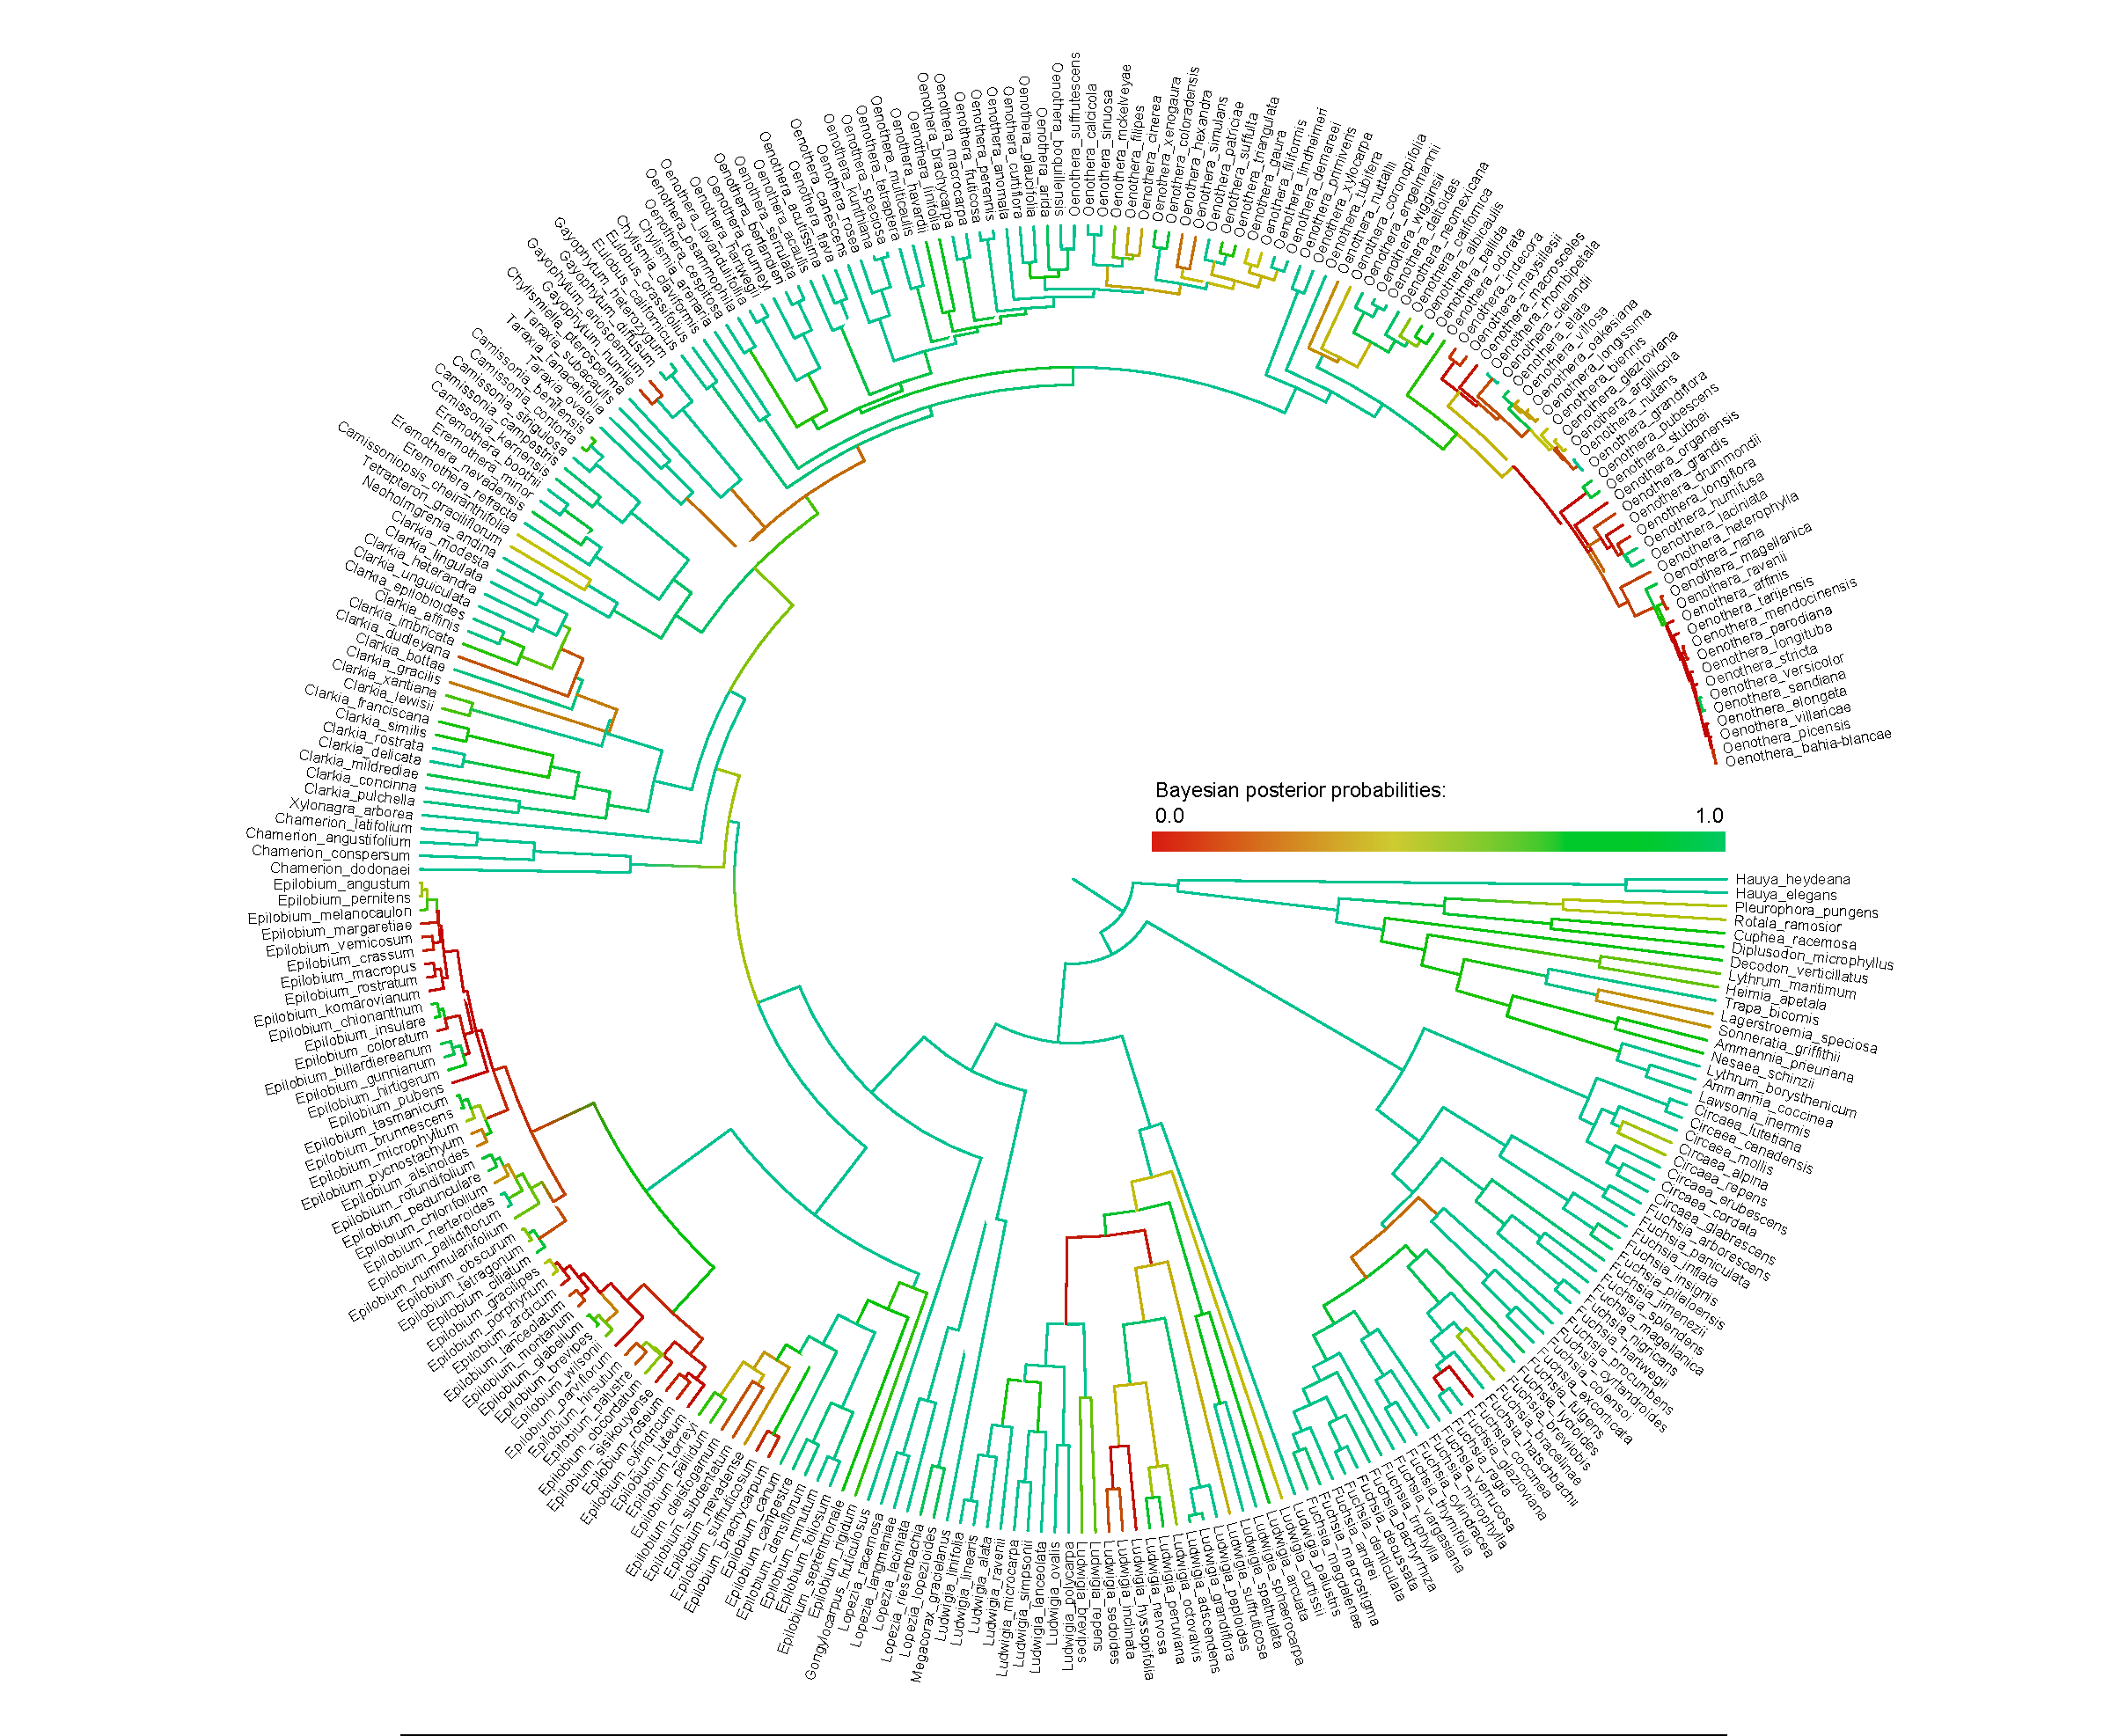
\includegraphics[width=1.6\linewidth, trim=0 10 0 0, clip=true]{colored_posterior}
    }
    \caption{Phylogeny blah blah blah}
    \label{posteriors}
\end{figure*}

\begin{figure*}[p]
    \vspace*{-2cm}
    \makebox[\linewidth]{
        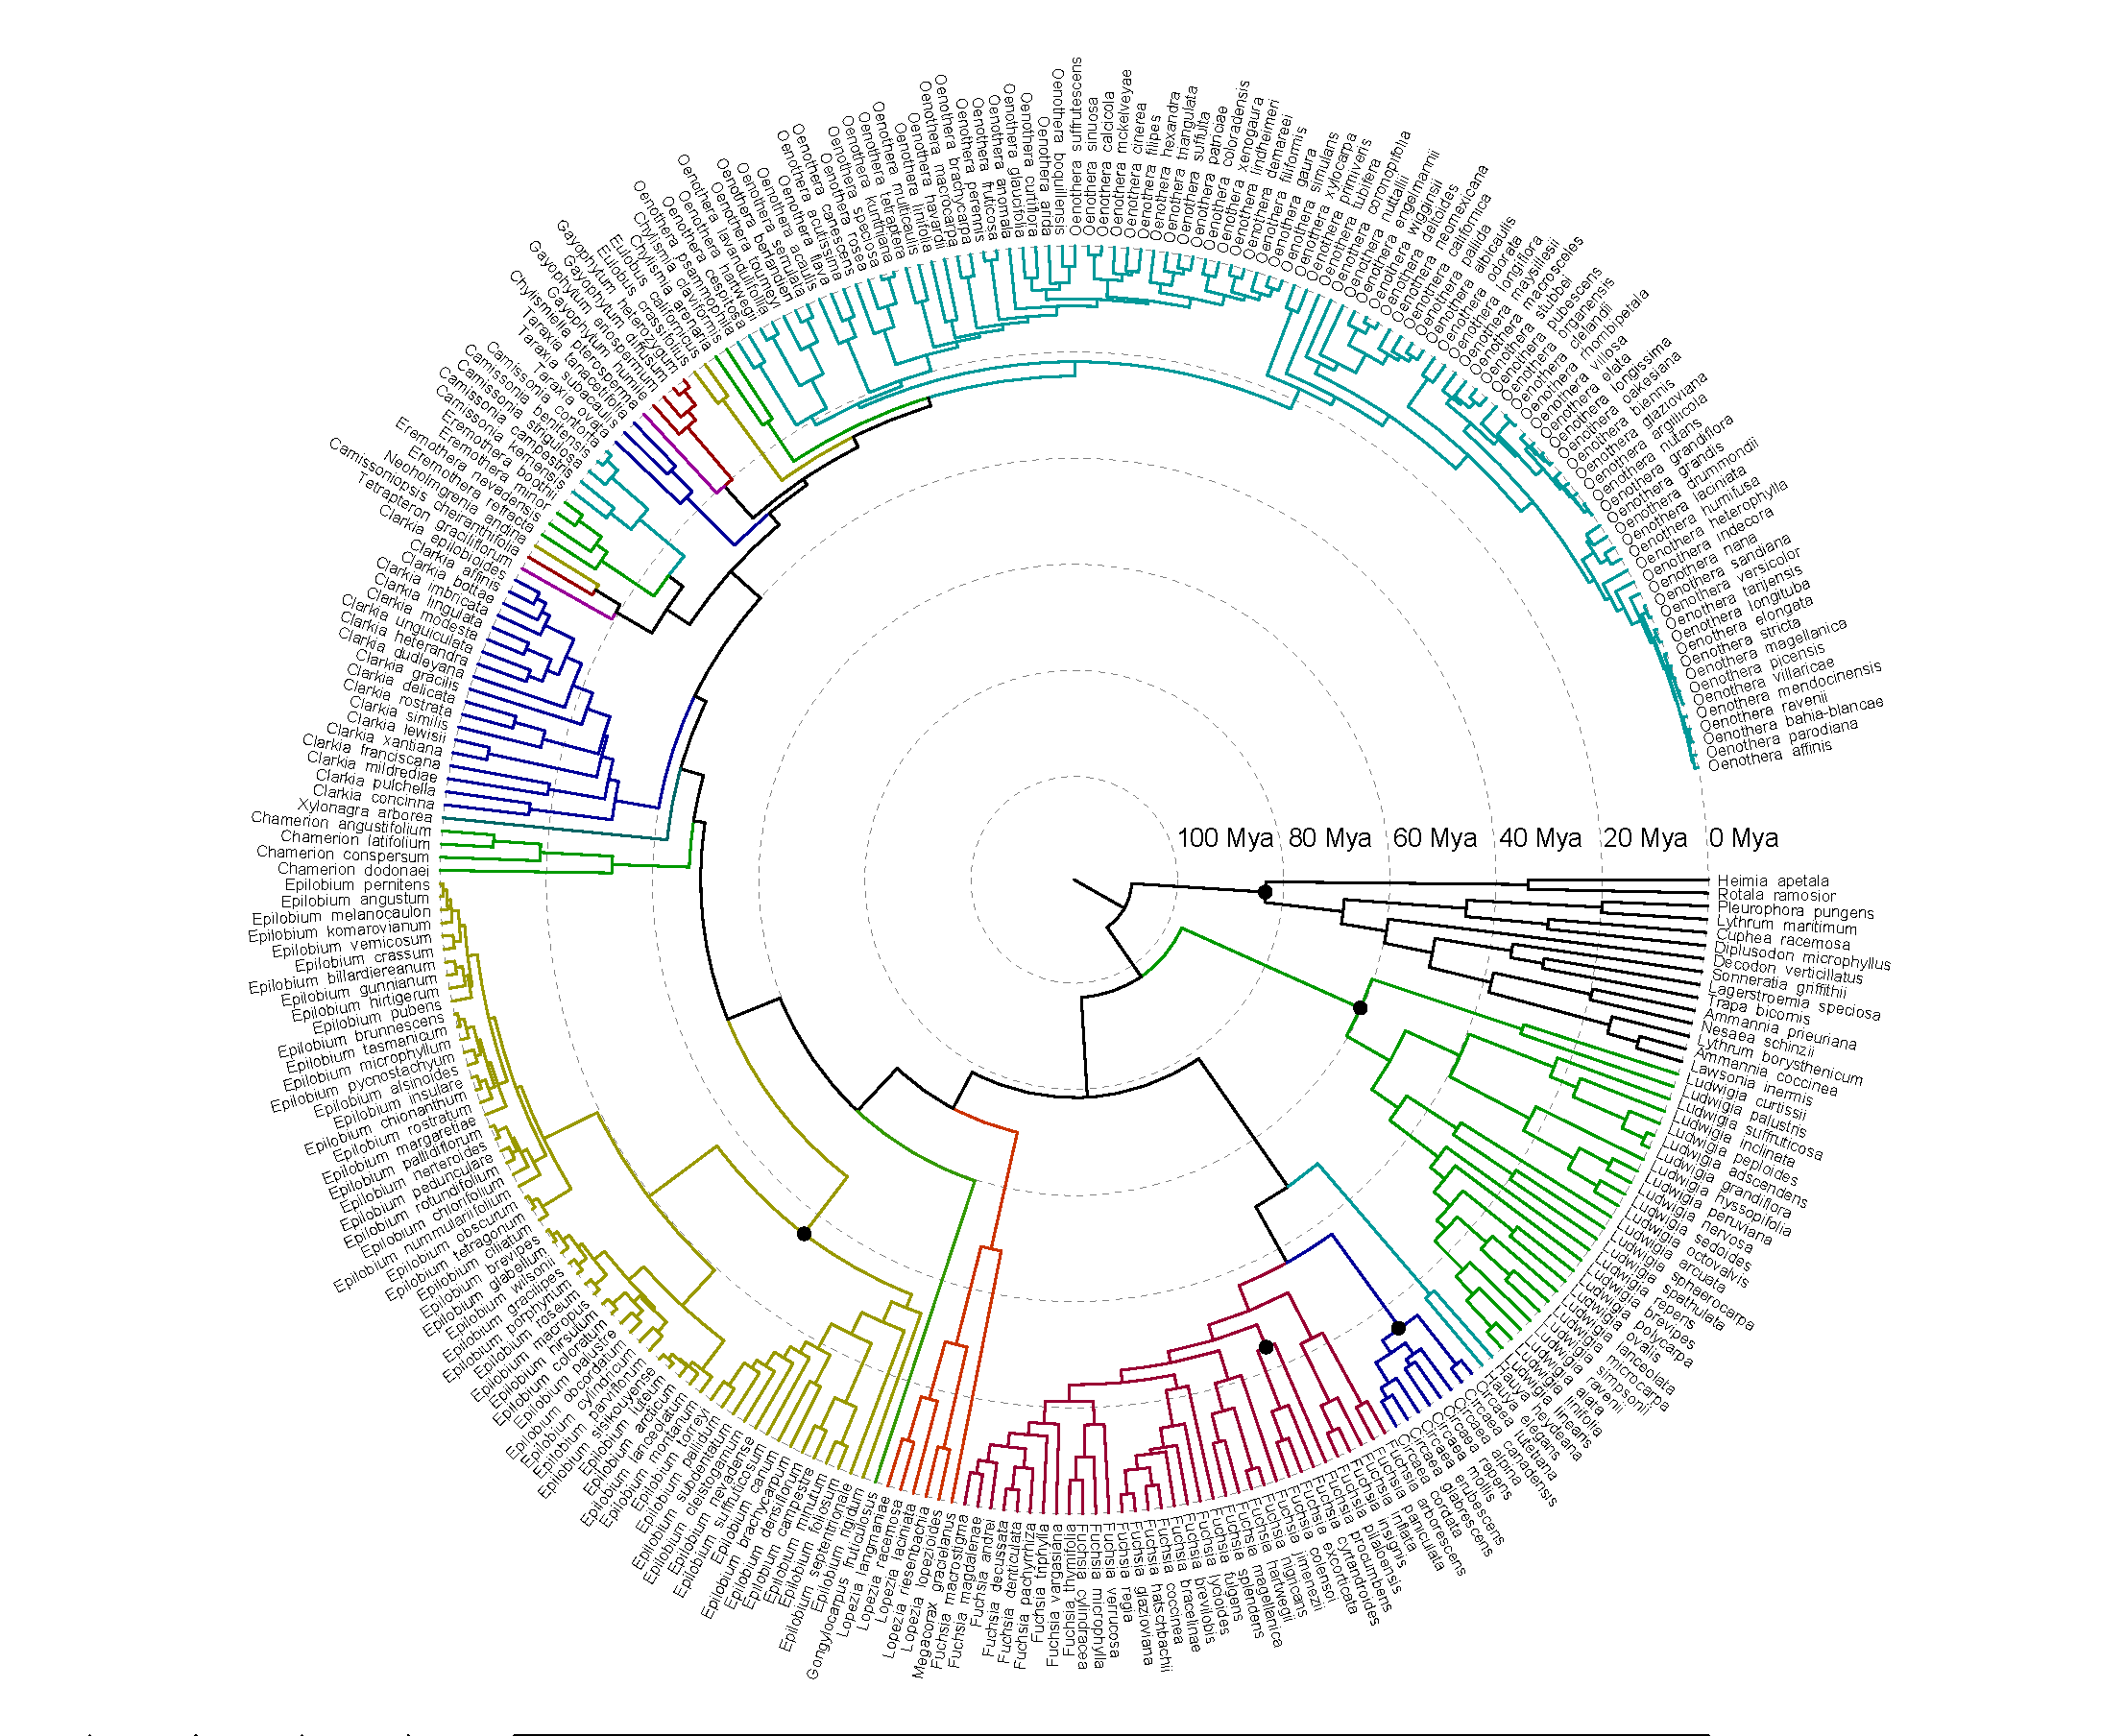
\includegraphics[width=1.6\linewidth, trim=0 10 0 0, clip=true]{time_colored_genera}
    }
    \caption{Sequence diagram}
    \label{genera}
\end{figure*}

%%%%%%%%%%%%%%%%%%%%%%%
%% conclusion
%%%%%%%%%%%%%%%%%%%%%%%

\section{Conclusion}

blah blah


%%%%%%%%%%%%%%%%%%%%%%%
%% references
%%%%%%%%%%%%%%%%%%%%%%%

\section*{References}

\bibliography{manuscriptbib}

\end{document}
